\documentclass[12pt]{article}
\usepackage{polish}
\usepackage[utf8]{inputenc}
\usepackage{url}
\usepackage{hyperref}
\usepackage{multicol}
\usepackage{geometry}
\usepackage{fancyhdr}
\usepackage{graphicx}
\usepackage{enumitem}

\setlist[itemize]{noitemsep, topsep=5pt}
\geometry{a4paper,total={170mm,257mm},left=20mm,top=20mm}

\graphicspath{ {../} }

\pagestyle{fancy}
\rhead{Raport}
\lhead{}
\cfoot{}
\rfoot{Strona \thepage}
\fancypagestyle{firststyle}
{
\fancyhf{}
\fancyfoot[R]{Strona \thepage}
}

\newcounter{coun}[section]
\newenvironment{coun}[1][]{\refstepcounter{coun}\par\medskip
{\noindent\textbf{\thecoun #1. }}\leftskip=0em\rightskip=0em }{\par\medskip}

\begin{document}
\title{Raport \\  (środowisko agenta i reprezentacja wiedzy)}
\author{Marcin Woźniak \\ Filip Izydorczyk \\ Hubert Wrzesiński \\ Przemysław Fierek\\ \\ \textbf{Grupa 5} }
\maketitle
\thispagestyle{firststyle}
\vspace{10}
Repozytorium: \url{https://github.com/linux923344/autonomiczny_saper/}} \\

Spis klas użytych w projekcie:
\begin{enumerate}
	\item {\textbf{Board} - jako argumenty przyjmuje X i Y, które są rozmiarem renderowanego okna. Klasa odpowiada za renderowanie mapy i zarządzanie obiektami na niej.}
	\item {\textbf{Bomb} (BombRed, BombBlue, BombYellow) - obiekt odpowiedzialny za renderowanie oraz logikę bomby}
	\item{\textbf{Direction} - enum, który daje nam informacje, w którym kierunku ma się poruszać postać.}
	\item{\textbf{MapReader} - argumentem przy jej tworzeniu jest plansza czyli obiekt typu Board, na której MapReader będzie tworzył obiekty które są przechowywane w zewnętrznym pliku.}
	\item{\textbf{Stone} - klasa, która jest odpowiedzialna za informacje potrzebne do wyrenderowania kamienia.}
	\item{\textbf{Tool} - klasa, która jest odpowiedzialna za informacje potrzebne do wyrenderowania narzędzia.}
	\item{\textbf{Saper} - przechowuje informacje potrzebne do wyrenderowania Sapera, co posiada w ekwipunku oraz jakie zadania musi wykonać.}
	\item{\textbf{PathFinder} - tworzy klasę typu Graph na podstawie podanego Boarda}
	\item{\textbf{Graph} - klasa znajduje ścieżkę w grafie do danego punktu i zwraca listę kierunków, w jakich musi poruszać się postać aby dojść do danego punktu.}
\end{enumerate}
\newpage 

\noindent\textbf{27.03.2019 r.}
\setcounter{coun}{0}\\
\coun {Zaprojektowanie diagramu klas.}\\
\begin{center}
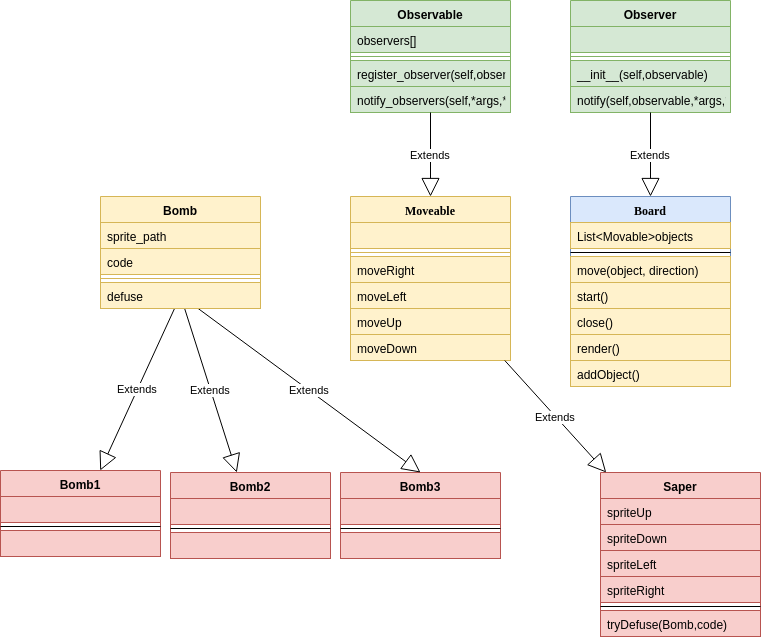
\includegraphics[scale=0.47]{logika.png}
\end{center}
\coun {Na podstawie diagramu, została stworzona klasa główna oraz jej podklasy.}
\coun {Został stworzony szablon planszy razem z umieszczonymi na niej bombami. }
\begin{center}
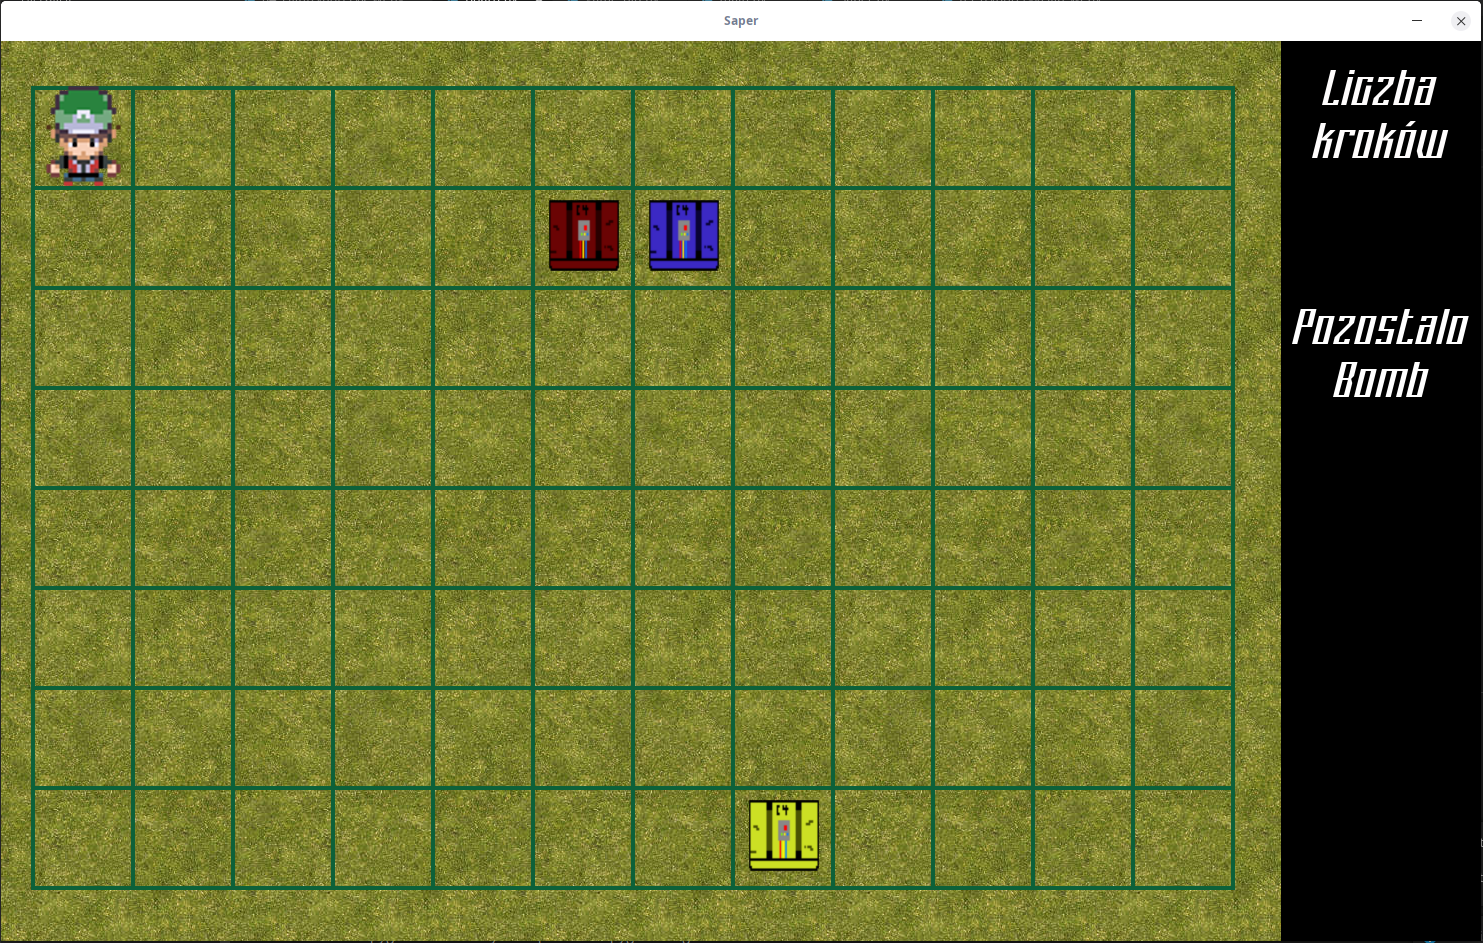
\includegraphics[scale=0.35]{plansza.png}
\end{center}
Na załączonym zrzucie ekranu widoczny jest saper czyli nasz Agent, oraz trzy kolorowe obiekty (bomby), które nasz agent ma za zadanie je rozbroić.\\

\noindent\textbf{10.04.2019 r.}\\
\setcounter{coun}{0}

W tym dniu została dokończona reprezentacja wiedzy w naszym projekcie.
Przedstawimy ją teraz:

\coun{Posiadamy trzy rodzaje bomb (czerwona, żółta, niebieska).}
\coun{Aby rozbroić bombę czewoną musimy posiadać narzędzie dodatkowo zmieścić się w wyznaczonym czasie. Jednostką czasu w naszym świecie jest jeden krok.}
\coun{Aby rozbroić pozostałe bomby Saper musi tylko do nich podejść, oczywiście jak nakrótszym czasie.}
\coun{Saper będzie wyznaczał drogę za pomocą algorytmu przeszukiwania grafu.}\\

\noindent\textbf{15.04.2019 r.}
\setcounter{coun}{0}\\

W tym dniu został zaimplementowany wyznaczanie ścieżki za pomocą algorytmu przeszukiwania DFS oraz kilka klas.\\

\noindent\textbf{17.04.2019 r.}
\setcounter{coun}{0}\\

Spisanie raportu i wypisanie wszystkich klas znajdujących się w projekcie.\\

\noindent\textbf{30.04.2019 r.}
\setcounter{coun}{0}\\

Dodanie ekwipunku i ustalenie zasad działania bomb. Bomby będą miały określony czas, a narzędzia będą potrzebne do rozbrojenia ich. \\

\noindent\textbf{6.05.2019 r.}
\setcounter{coun}{0}\\

Implementacja algorytmu BFS. \\ 

\noindent\textbf{14.05.2019 r.}
\setcounter{coun}{0}\\

Implementacja algorytmu Best-First Search. \\

\end{document}

